\documentclass[
    11pt,
    latin1,
    a4paper,
    %titelpage,
    oneside
]{scrreprt}
\usepackage[latin1]{inputenc}
\usepackage[ngerman]{babel}
\usepackage[T1]{fontenc}
\usepackage{lmodern}
\usepackage{ngerman}
\usepackage{scrpage2}
\usepackage{pdfpages}
\usepackage{lastpage}
\usepackage{caption}
\usepackage[noindentafter]{titlesec}
\usepackage{textcomp}
\usepackage{graphicx}
\usepackage{wrapfig}
\usepackage{subfigure}
\usepackage{float}
\usepackage{url}
\usepackage{hyperref}
\usepackage{setspace}
\usepackage{amsmath}
\usepackage{booktabs}
\usepackage{ifthen}
\usepackage{pstricks,pst-uml}

% ========== OWL CLASS SIMPLIFICATION ==========
\newcommand{\OWLRoot}[2]{%
\rput[l](#1) {%
  \rnode{#2} { \umlClass{#2}{} }%
}}
\newcommand{\OWLClass}[3]{%
\rput[l](#1) {%
  \rnode{#2} { \umlClass{#2}{} }%
  \ncSE{#3}{#2}%
  \ncputicon{umlHerit}%
}}

% ========== CODEBLOCKS FORMATTING ==========
\usepackage{listings}
\usepackage{color}
\definecolor{listings}{RGB}{237,241,246}
\lstloadlanguages{Clean,sh,bash,[ANSI]C,[ISO]C++,SQL,Pascal,Python,PHP,[gnu]awk,XML,XSLT,HTML}
\lstset{language=Clean,frame=tb,numbers=left,captionpos=b,numberstyle=\tiny,basicstyle=\small,breaklines=true}
\renewcommand*{\thelstnumber}{{\the\value{lstnumber}}{:}}
\renewcommand*{\lstlistlistingname}{Codeblock-Verzeichnis}
\renewcommand*{\lstlistingname}{Codeblock}

% ========== INDEX ==========
\usepackage{makeidx}
\renewcommand{\indexname}{Stichwortverzeichnis}
\makeindex
\let\oldemph=\emph
\renewcommand{\emph}[1]{\index{#1}\oldemph{#1}}

% ========== SPECIAL NOMENCLATURE ==========
%% see http://blog.stefan-macke.com/2006/05/03/abkurzungsverzeichnis-mit-latex/
%% and http://my.opera.com/timomeinen/blog/show.dml/68644
\usepackage{nomencl}
\let\abbrev\nomenclature
\renewcommand{\nomname}{Abk\"urzungsverzeichnis}
\setlength{\nomlabelwidth}{.25\hsize}
\renewcommand{\nomlabel}[1]{#1 \dotfill}
\setlength{\nomitemsep}{-\parsep}
\makeglossary

% ========== Caption modifications ==========
\usepackage{caption}
\captionsetup{margin=20pt,labelfont=bf,font=footnotesize,justification=justified,singlelinecheck=false}

% ========== PDF META-INFORMATION ==========
\hypersetup{%
        bookmarks=true, % Lesezeichen erzeugen
        bookmarksopen=false, % Lesezeichen ausgeklappt
        bookmarksnumbered=true, % Anzeige der Kapitelzahlen am Anfang der Namen der Lesezeichen
        breaklinks=true, % ermöglicht einen Umbruch von URLs
        colorlinks=true, % Einfärbung von Links
        linkcolor=black, % Linkfarbe
        anchorcolor=black, % Ankerfarbe
        citecolor=blue, % Literaturlinks
        filecolor=black, % Links zu lokalen Dateien
        menucolor=black, % Acrobat Menü Einträge
        urlcolor=blue, % URL-Farbe
        %pdfpagemode=UseThumbs, % Anzeige der Piktogramme
        pdfstartpage={1}, % Startseite
        pdftitle = {Dokumentation zu KnowNet},
        pdfsubject = {KnowNet ist eine Ontologie und darauf basierende Suchmaschine für Dokumente und Aussagen},
        pdfauthor = {Lukas Zurschmiede},
        pdfkeywords = {Knowledge, Network, Ontology, KnowNet, Pirateparty, search, searchengine, nowledgebase},
        pdfcreator = {LaTeX to PDF-Creator},
        pdfproducer = {LaTeX with hyperref}
}

% ========== GLOBALS ==========
\setcounter{tocdepth}{2}
\setcounter{secnumdepth}{2}
\bibliographystyle{alphadin}
\newcommand{\at}{\symbol{64}}
\newcommand{\tld}{\symbol{126}}

% ========== META-INFORMATION ==========
\author{Lukas Zurschmiede\\Bachelor of Science in Information technology}
\date{Lommis, 21. Juni 2012}
\publishers{Lukas Zurschmiede\\Pirateparty Switzerland}
\titlehead{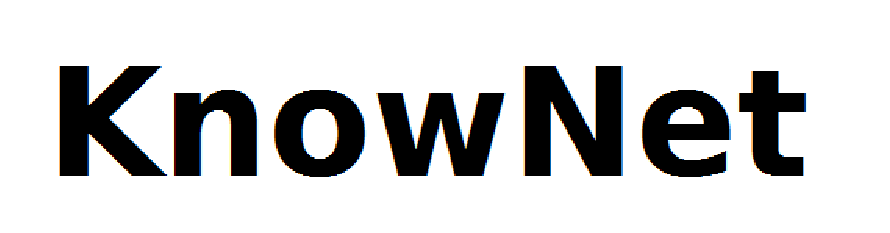
\includegraphics{images/knownet_logo.eps}}
\title{KnowNet, eine Ontologie und Suchmaschine f\"ur Dokumente und Statements}
\subject{Idee f\"ur eine Software\\
Piratenpartei Schweiz}

\begin{document}

\maketitle

\newpage
\singlespacing
\tableofcontents

\pagebreak
\onehalfspacing
\setcounter{page}{1}
\pagenumbering{arabic}

\chapter{Einleitung} \label{sec:introduction}

\section{Die Idee \emph{KnowNet}}

\emph{KnowNet} - Knowledge Network - ist prim\"ar eine Ontologie, welche Dokumente von und \"uber eine politische Partei sammelt und entsprechend aufbereitet anbietet. Die Idee dahinter ist, dass man durch eine einfache, eventuell neuartige Suchoberfl\"ache, Aussagen und Meinungen aber auch Dokumente von einer Partei, respektive \"uber eine Partei finden kann. Eine Partei kann Unterparteien (Sektionen) aufweisen, welche somit bei einem lokalen Thema die Ontologie abfragen k\"onnen, ob zu diesem Thema schon ein Statement oder Dokument vorhanden ist respektive ob eine andere Sektion schon etwas dar\"uber gesagt hat, aber auch, ob es eventuell andere Organisatinen wie Medienh\"auser gibt, welche der Partei eine Aussage diesbez\"uglich unterstellt haben.

Die Ontologie soll schlussendlich eine einfache M\"oglichkeit bieten, Dinge \"uber eine komplexe Struktur zu erfahren um daraus Schlussfolgerungen und Thesen auf zu stellen, jedoch auch um heraus zu finden, ob denn schon eine der Sektionen eine Meinung oder Aussage \"uber ein gewisses Thema gemacht hat.

\section{Fakten \"uber die Ontologie} \label{sec:facts}

Die Ontologie kann durch folgende Aussagen beschreiben werden:

\begin{itemize} \setlength{\itemsep}{0cm}
  \item Die Ontologie besteht haupts\"achlich aus Dokumenten, Personen, Organisationen und Vereinen;
  \item Ein Dokument kann ein (Positions-)Papier, ein Statement oder ein Journalistisches Werk sein;
  \item Ein Verein kann Untervereine haben - und somit auch \"Ubergeordnete;
  \item Eine Person kann einem oder mehreren Vereinen angeh\"oren;
  \item Ist eine Person Mitglied eines Vereines, kann Sie deren Meinung \"offentlich vertreten;
  \item Eine Person kann einen oder mehrere Berufe aus\"uben;
  \item Eine Person kann in einer oder mehreren Organisationen arbeiten;
  \item Ein Dokument das einem Verein zugeordnet ist, beschreibt deren Ansichten;
  \item Ein Dokument das einer Organisation zugeordnet ist, beschriebt die Ansicht dieser \"uber einen Vereins;
  \item Ein Dokument ist von mindestens einer Person geschrieben;
  \item Ein Dokument besteht aus S\"atzen;
  \item Ein Satz besteht aus W\"ortern;
  \item Ein Word ist eine Abfolge von Zeichen;
  \item Ein Wort kann aus mehreren anderen W\"ortern zusammengesetzt sein;
  \item Ein Wort kann in verschiedenen Sprachen vorkommen (\"Ubersetzungen);
  \item Ein Wort kann verschiedene Bedeutungen haben (Synonyme);
  \item Eine Person wird durch den Namen, Vornamen und den Nickname identifiziert;
  \item Eine Person muss mindestens eine Sprache sprechen;
  \item Ein Wort ist immer genau einer Sprache zugeordnet;
  \item Ein Dokument ist immer genau einer Sprache zugeordnet;
\end{itemize}

\section{Struktur und Aufbau} \label{sec:structure}

Es bietet sich an, \emph{KnowNet} durch eine Ontologie ab zu bilden. Ontologien die auf dem OWL-Standard\cite{W3COWL} basieren, bieten die M\"oglichkeit, mittels einer in den Grundz\"ugen einfachen Sprache eine Wissensdatenbank komplex verkn\"upft zu speichern und verwalten. OWL ist eine Erweiterung von RDF/S und ist, wie RDF auch, durch die zwei Syntaxen, \emph{Turtle} respektive \emph{N3} und \emph{XML}, definiert. Obwohl \emph{XML} im Vergleich zu \emph{Turtle} einiges mehr "'drum herum"` hat, ist es dennoch einfacher zu erstellen und auch zu pflegen als \emph{Turtle}. Auch kann die Ontologie in dieser Syntax durch andere Programme einfacher gelesen werden und ist auch einfacher wartbar, da Syntaxfehler durch gute Editoren schneller erkannt werden respektive das ganze in enem Browser betrachtet werden kann.

OWL ist zur Zeit in Version 1 und in Version 2 definiert. Der OWL 2 Standard\cite{W3COWL2} ist komplett R\"uckw\"artskompatibel zu OWL 1, enth\"allt jedoch Erweiterungen, welche in der Ursprungsversion schlicht gefehlt haben. Einige der Neuerungen sind rein syntaktischer Natur, andere sind Funktionen und Features, welche bislang gefehlt haben. Die Ontologie f\"ur \emph{KnowNet} wird noch mit OWL 1 implementiert, da nicht klar zu sehen ist, ob die verwendeten Libraries (siehe \nameref{sec:technologies} auf Seite \pageref{sec:technologies}) auch OWL 2 verstehen. Dies muss in einem kurzen Test gepr\"uft werden und anschliessend gegebenenfals die Ontologie nach OWL 2 gewandelt werden, wenn dies denn ben\"otigt wird.

\subsection{Technologien} \label{sec:technologies}

Es werden Folgende Technologien und Standards verwendet:

\begin{description}
  \item[Ontologie] OWL 1, Subsprache OWL DL (Description Logic), als Ontologiebeschreibungssprache
  \item[Abfragen] SPARQL\cite{SPARQL} zur Ontologie, JSON evtl. auch XML als Client-Server Kommunikation
  \item[Programmierung] C/C++ mit Qt4\cite{QT} (je nach Erscheinungsdatum auch schon Qt5)
  \item[Eventuell] HTML 5, Javascript als Client oder zur Abfrage mittels REST/JSON/XML
  \item[Libraries] Redland RDF Libraries\cite{LIBRDF}
  \item[Datenbank] PostgreSQL und MySQL Serverseitig, SQLite zum Entwickeln und eventuell auf dem Client wenn notwendig
\end{description}

Die Liste ist offen und wird entsprechend angepasst wenn bei der Entwicklung und/oder Planung gemerkt wird, dass andere Dinge und Libraries eingesetzt oder nicht verwendet werden.

\chapter{Aufbau der Ontologie} \label{sec:ontology}

% ========== CLASSES ==========

\section{Klassen} \label{sec:class}

Folgende Klassen und Spezialisierungen werden f\"ur die Ontologie gebraucht. In den nachfolgenden Kapiteln werden diese noch genauer beschrieben. Die Verlinkungen zwischen den einzelnen Klassen, also die ObjectProperties, werden im Kapitel \nameref{sec:relations} auf Seite \pageref{sec:relations} beschrieben. In den jeweiligen Detailbeschreibungen der Klassen wird jeweils darauf eingegangen und darauf verwiesen. Die Datenfelder, also die DataProperties, werden in den Detailbeschreibungen der Klassen jedoch auch im Kapitel \nameref{sec:datatypes} auf Seite \pageref{sec:datatypes} beschrieben.

\begin{figure}[H]
\centering
\begin{pspicture}(10,15)

\OWLRoot{0,14.5}{Thing}
\OWLClass{3,13}{Word}{Thing}
\OWLClass{3,12}{Sentence}{Thing}
\OWLClass{3,11}{Translation}{Thing}
\OWLClass{3,10}{Synonym}{Thing}
\OWLClass{3,9}{Document}{Thing}
\OWLClass{6,7.5}{Paper}{Document}
\OWLClass{6,6.5}{Statement}{Document}
\OWLClass{6,5.5}{Journal}{Document}
\OWLClass{3,4}{Person}{Thing}
\OWLClass{3,3}{Profession}{Thing}
\OWLClass{3,2}{Organization}{Thing}
\OWLClass{3,1}{Association}{Thing}

\end{pspicture}
\label{owl:main}
\caption{Die OWL-Klassen und deren Abh\"angigkeiten im \"Uberblick}
\end{figure}


\begin{table}[H]
  \centering
  \begin{tabular}{ | l | p{4cm} | l | l| }
    \hline
    \textbf{Class} & \textbf{Beschreibung} & \textbf{SubClass of} & \textbf{Details} \\ \hline
    \textbf{Word} & Beschreibt ein einzelnes Wort in einer Sprache; Es kann aus mehreren W\"ortern zusammengesetzt sein sowie \"Ubersetzungen und Synonyme aufweisen; & Thing & \nameref{sec:class_word}, Seite \pageref{sec:class_word} \\ \hline
    \textbf{Translation} & Gruppiert die gleichen W\"orter aus verschiedenen Sprachen & Thing & \nameref{sec:class_translation}, Seite \pageref{sec:class_translation} \\ \hline
    \textbf{Synonym} & Gruppiert unterschiedliche W\"orter der gleichen Sprache mit der gleichen Bedeutung & Thing & \nameref{sec:class_synonym}, Seite \pageref{sec:class_synonym} \\ \hline
    \textbf{Sentence} & Ein Satz besteht aus verschiedenen W\"ortern & Thing & \nameref{sec:class_sentence}, Seite \pageref{sec:class_sentence} \\ \hline
    \textbf{Document} & Ein Dokument besteht aus verschiedenen S\"atzen & Thing & \nameref{sec:class_document}, Seite \pageref{sec:class_document} \\ \hline
    \textbf{Paper} & Ein Positionspapier/Dokument einer Partei & Document & \nameref{sec:class_paper}, Seite \pageref{sec:class_paper} \\ \hline
    \textbf{Statement} & Eine Aussage eines Parteimitgliedes & Document & \nameref{sec:class_statement}, Seite \pageref{sec:class_statement} \\ \hline
    \textbf{Journal} & Ein Zeitungsbericht \"uber eine Partei & Document & \nameref{sec:class_journal}, Seite \pageref{sec:class_journal} \\ \hline
    \textbf{Person} & Eine Person im Allgemeinen & Thing & \nameref{sec:class_person}, Seite \pageref{sec:class_person} \\ \hline
    \textbf{Profession} & Beschreibt einen Beruf, welchen eine Person aus\"uben kann & Person & \nameref{sec:class_profession}, Seite \pageref{sec:class_profession} \\ \hline
    \textbf{Organization} & Eine Organisation welche Journalistische Werke herstellt/verbreitet & Thing & \nameref{sec:class_organization}, Seite \pageref{sec:class_organization} \\ \hline
    \textbf{Association} & Eine (politische) Partei, welche Mitglieder und Angestellte haben kann & Thing & \nameref{sec:class_association}, Seite \pageref{sec:class_association} \\ \hline
  \end{tabular}
  \caption{\"Ubersicht und kurze Beschreibung \"uber alle Klassen der Ontologie}
  \label{tbl:classes}
\end{table}


\subsection{Klasse: Word} \label{sec:class_word}

Die Klasse \emph{Word} wird verwendet, um ein einzelnes Wort, welches innerhalb eines Dokumentes gefunden werden soll, zu definieren. Bei zusammengesetzten W\"ortern kann mit der Relation \emph{contains-word} (siehe \nameref{sec:rel_containsword} Seite \pageref{sec:rel_containsword}) angegeben werden, welche einzelnen W\"orter in diesem Wort vereint sind. Durch das Datenfeld \emph{lang} (siehe \nameref{sec:data_lang} Seite \pageref{sec:data_lang}) wird die Sprache des jeweiligen Wortes in iso639-1 (zwei Zeichen) definiert. Um \"Ubersetzungen miteinander zu verkn\"upfen, wird die Klasse \emph{Translation} (siehe \nameref{sec:class_translation} Seite \pageref{sec:class_translation}) verwendet.

Durch die Relation \emph{wordtype} (siehe \nameref{sec:data_wordtype} Seite \pageref{sec:data_wordtype}) wird die Art des Wortes definiert, also ob es sich um ein Nomen, ein Adjektiv oder ein Verb handelt. Dadurch kann bei der Suche explizit nach Eigenschaften oder Aktionen gesucht werden, welche ein Dokument beschreibt.

\subsubsection{Code}  \label{sec:class_word_code}

\begin{figure}[H]
 \lstset{language=XML}
 \begin{lstlisting}[label=owl:word,caption={Die Klasse \emph{Word} beschreibt ein einzelnes Wort}]
<owl:Class rdf:ID="Word">
</owl:Class>
 \end{lstlisting}
\end{figure}


\subsection{Klasse: Translation} \label{sec:class_translation}

Die Klasse \emph{Translation} ist eine Vereinigung aller W\"orter in verschiedenen Sprachen mit der selben Bedeutung. Dies geschieht durch die Angabe \texttt{owl:minCardinality}, welche aussagt, dass eine \"Ubersetzung mindestens zwei W\"orter in der Range des Properties \emph{is-same} (siehe \nameref{sec:rel_issame} Seite \pageref{sec:rel_issame}) aufweisen muss. Durch dieses Konstrukt k\"onnen neue W\"orter einfach und schnell eingepflegt und als \"Ubersetzung definiert werden ohne die W\"orter selber zu manipulieren, sowie bei einer Abfrage in der Liste gesucht werden.

\subsubsection{Code}  \label{sec:class_translation_code}

\begin{figure}[H]
 \lstset{language=XML}
 \begin{lstlisting}[label=owl:translation,caption={Die Klasse \emph{Translation} beinhaltet alle \"Ubersetzungen eines Wortes}]
<owl:Class rdf:ID="Translation">
  <rdfs:subClassOf>
    <owl:Restriction>
      <owl:onProperty rdf:resource="#is-same" />
      <owl:minCardinality rdf:datatype="&xsd;nonNegativeInteger">2</owl:minCardinality>
    </owl:Restriction>
  </rdfs:subClassOf>
</owl:Class>
 \end{lstlisting}
\end{figure}


\subsection{Klasse: Synonym} \label{sec:class_synonym}

Die Klasse \emph{Synonym} dient zur Verkn\"upfung mehrerer W\"ortern mit der gleichen Bedeutung. Dies geschieht durch die Angabe \texttt{owl:minCardinality}, welche aussagt, dass ein Synonym mindestens zwei W\"orter in der Range des Properties \emph{means-same} (siehe \nameref{sec:rel_meanssame} Seite \pageref{sec:rel_meanssame}) aufweisen muss. Durch dieses Konstrukt k\"onnen neue W\"orter einfach und schnell eingepflegt und als Synonyme von anderen definiert werden, ohne die W\"orter selber zu manipulieren, sowie bei einer Abfrage in der Liste gesucht werden.

\subsubsection{Code}  \label{sec:class_synonym_code}

\begin{figure}[H]
 \lstset{language=XML}
 \begin{lstlisting}[label=owl:synonym,caption={Die Klasse \emph{Synonym} beinhaltet alle W\"orter dir etwas \"ahnliches bedeuten}]
<owl:Class rdf:ID="Synonym">
  <rdfs:subClassOf>
    <owl:Restriction>
      <owl:onProperty rdf:resource="#means-same" />
      <owl:minCardinality rdf:datatype="&xsd;nonNegativeInteger">2</owl:minCardinality>
    </owl:Restriction>
  </rdfs:subClassOf>
</owl:Class>
 \end{lstlisting}
\end{figure}


\subsection{Klasse: Sentence} \label{sec:class_sentence}

Ein Satz, welcher durch die Klasse \emph{Sentence} definiert wird, ist eine Vereinigung von W\"ortern zu einer Gruppe von solchen. Die Reihenfolge der W\"orter ist dabei egal, es geht nur um das Zusammenspiel und den Zusammenhang einzelner W\"orter und dessen Bedeutung. Dieses Konstrukt wird bei der Instanz durch das Property \emph{has-word} (siehe \nameref{sec:rel_hasword} Seite \pageref{sec:rel_hasword}) mittels einer anonyme Klasse mit \texttt{owl:unionOf} definiert.

\subsubsection{Code}  \label{sec:class_sentence_code}

\begin{figure}[H]
 \lstset{language=XML}
 \begin{lstlisting}[label=owl:sentence,caption={Die Klasse \emph{Sentence} f\"ugt einzelne \emph{Word}-Instanzen zu einem Satz zusammen}]
<owl:Class rdf:ID="Sentence">
  <rdfs:subClassOf>
    <owl:Restriction>
      <owl:onProperty rdf:resource="#has-word" />
      <owl:someValuesFrom ref:resource="#Word" />
    </owl:Restriction>
  </rdfs:subClassOf>
</owl:Class>
 \end{lstlisting}
\end{figure}


\subsection{Klasse: Document} \label{sec:class_document}

Die Klasse \emph{Document} ist, \"ahnlich wie \emph{Sentence}, eine Kombination von verschiedenen S\"atzen. Die Reihenfolge dieser spielt keine Rolle, es geht rein um den logischen Zusammenhang der einzelnen S\"atze und somit der verschiedenen W\"orter.

ToDo:
\textbb{Anmerkung:} Eventuell macht es Sinn, ein Dokument noch durch Kapitel zu strukturieren. Dies k\"onnte durch eine Relation "'ein Dokument aus Dokumenten"` sowie der Angabe eines Satzes als \"Uberschrift erreicht werden. Die Frage ist nur, inwieweit sich diese Komplexit\"atssteigerung rechtfertigen w\"urde.

\subsubsection{Code} \label{sec:class_sentence_code}

\begin{figure}[H]
 \lstset{language=XML}
 \begin{lstlisting}[label=owl:document,caption={Die Klasse \emph{Document} f\"ugt einzelne S\"atze zu einem Dokument zusammen}]
<owl:Class rdf:ID="Document">
  <rdfs:subClassOf>
    <owl:Restriction>
      <owl:onProperty rdf:resource="#has-sentence" />
      <owl:someValuesFrom ref:resource="#Sentence" />
    </owl:Restriction>
  </rdfs:subClassOf>
</owl:Class>
 \end{lstlisting}
\end{figure}


\subsection{Klasse: Paper} \label{sec:class_paper}

Die Klasse \emph{Paper} ist eine Unterklasse von \emph{Document} und definiert ein Dokument, welches im Zusammenhang zu einem Verein, also der Klasse \emph{Association} steht. Durch diese Unterklasse kann besser nach Dokumenten gesucht werden, welche von einer bestimmten politischen Partei oder einer Sektion von dieser, verfasst wurden. Ein Dokument, welches durch diese Klasse implementiert ist, beschreibt in den meisten F\"allen ein Positionspapier oder \"ahnliches.

Neuigkeiten, Stellungnahmen, Pressetexte, Communiques etc. sollten als \emph{Statement} definiert werden und nicht als \emp{Paper}.

\subsubsection{Code} \label{sec:class_paper_code}

\begin{figure}[H]
 \lstset{language=XML}
 \begin{lstlisting}[label=owl:paper,caption={Die Klasse \emph{Paper} ist ein Dokument einer \emph{Association}, also eines partei/Gesellschaft}]
<owl:Class rdf:ID="Paper">
  <rdfs:subClassOf rdf:resurce="#Document" />
</owl:Class>
 \end{lstlisting}
\end{figure}


\subsection{Klasse: Statement} \label{sec:class_statement}

Die Klasse \emph{Statement} ist eine Unterklasse von \emph{Document} und wird verwendet, um eine Aussage/Statement einer Person, Communiques und Pressetexte oder einfache Stellungnahmen, etc. zu deklarieren. Bei einem Statement muss bei der Suche unterschieden werden, ob dieses von einer Person aus der Klasse \emph{Association} stammt, oder von einer beliebigen anderen Person. Ein Statement von einer beliebigen Person kann zum Beispiel genutzt werden, um sich ein Bild \"uber eine Partei von Aussen zu machen, w\"ahrend eines von einer Person aus \emph{Association} genutzt werden kann, um sich ein Bild von innen zu machen.

Durch das Property \emph{from-text} (siehe \nameref{sec:res_fromtext} auf Seite \pageref{sec:res_fromtext}) kann ein Statement einem beliebigen anderen \emph{Document} zugeordnet werden. Dadurch kann ein Statement nicht nur als "'Aussage"` per se definiert werden, sondern auch als "'Zitat"` in anderen Dokumenten und Pressetexten markiert werden. Dadurch kann zum Beispiel die Attraktivit\"at und die Verbreitung gewisser Stellungnahmen gemesssen werden.

\subsubsection{Code} \label{sec:class_statement_code}

\begin{figure}[H]
 \lstset{language=XML}
 \begin{lstlisting}[label=owl:statement,caption={Ein \emph{Statement} beschreibt eine Aussage einer Person}]
<owl:Class rdf:ID="Statement">
  <rdfs:subClassOf rdf:resource="#Document" />
</owl:Class>
 \end{lstlisting}
\end{figure}


\subsection{Klasse: Journal} \label{sec:class_journal}

Ein \emph{Journal} ist eine Unterklasse von \emph{Document} und definiert einen Text, welcher von einem \emph{Journalist} geschrieben und von einer \emph{Organization} Ver\"offentlicht worden ist. Er stellt nicht die Meinung einer \emph{Association} dar, sondern diejenige eines Aussenstehenden. Ist der Author ebenfalls Mitglied der Klasse \emph{Member}, kann der Text jedoch als pers\"onliche Meinung und somit indirekt als Parteimeinung gedeutet werden.

Die texte der Klasse \emph{Journal} k\"onnen haupts\"achlich f\"ur ein Meinungsbild \"uber eine Partei hergenommen werden, bei welchem die Meinung von Aussen und nicht diejenige der Mitglieder z\"ahlt.

\subsubsection{Code} \label{sec:class_journal_code}

\begin{figure}[H]
 \lstset{language=XML}
 \begin{lstlisting}[label=owl:journal,caption={Ein \emph{Journal} ist ein Bericht \"uber eine \emph{Association}, welcher von einer \emph{Organization} herausgegeben wurde}]
<owl:Class rdf:ID="Journal">
  <rdfs:subClassOf rdf:resource="#Document" />
</owl:Class>
 \end{lstlisting}
\end{figure}


\subsection{Klasse: Person} \label{sec:class_person}

Die Klasse \emph{Person} wird verwendet, um irgend eine Person zu definieren. Dies kann ein Autor, ein Parteimitglied oder eine andere beliebige Person sein.

\subsubsection{Code} \label{sec:class_person_code}

\begin{figure}[H]
 \lstset{language=XML}
 \begin{lstlisting}[label=owl:person,caption={Die Klasse \emph{Person} definiert alle Personen}]
<owl:Class rdf:ID="Person">
</owl:Class>
 \end{lstlisting}
\end{figure}


\subsection{Klasse: Profession} \label{sec:class_profession}

Die Klasse \emph{Profession} wird verwendet, um einer \emph{Person} einen Beruf/Anstellung zuzuweisen. Dadurch kann man eventuell gewissen Berufsgruppen gewisse Meinungen zuweisen.

Die Zuweisung erfolgt durch die Relation \emph{working-as} (siehe \nameref{sec:rel_workingas} auf Seite \pageref{sec:rel_workingas}).

\subsubsection{Code} \label{sec:class_profession_code}

\begin{figure}[H]
 \lstset{language=XML}
 \begin{lstlisting}[label=owl:profession,caption={Die Klasse \emph{Caption} beschreibt jegliche Berufe}]
<owl:Class rdf:ID="Profession">
  <rdfs:subClassOf>
    <owl:Restriction>
      <owl:onProperty rdf:resource="#has-workers" />
      <owl:someValuesFrom ref:resource="#Person" />
    </owl:Restriction>
  </rdfs:subClassOf>
</owl:Class>
 \end{lstlisting}
\end{figure}


\subsection{Klasse: Organization} \label{sec:class_organization}

Die Klasse \emph{Organization} definiert die Arbeitgeber von \emph{Person}-Instanzen aber auch die Herausgeber von \emph{Journal}-Instanzen. Durch diese Zuweisung k\"onnen Aussagen und Meinungen, welche eine Zeitung von der Partei hat, eruiert werden. Eine \emph{Organization} kann mehrere Angestellte haben, welche nicht zwingendermassen nur bei der einen Organisation angestellt sind. Idealerweise besitzt die \emph{Person} ebenfalls das Attribut \emph{working-as} mit enem Verweis auf einen Beruf.

Eine Instanz kann nie gleichzeitig eine \emph{Organization} und eine \emph{Association} sein, diese zwei Klassen schliessen sich gegenseitig aus.

\subsubsection{Code} \label{sec:class_organization_code}

\begin{figure}[H]
 \lstset{language=XML}
 \begin{lstlisting}[label=owl:organization,caption={Die Klasse \emph{Organization} definiert einen Arbeitgeben, meistens ein Medienhaus}]
<owl:Class rdf:ID="Organization">
  <rdfs:subClassOf>
    <owl:Restriction>
      <owl:onProperty rdf:resource="#has-employee" />
      <owl:someValuesFrom ref:resource="#Person" />
    </owl:Restriction>
  </rdfs:subClassOf>
  <owl:disjointWith rdf:resource="#Association" />
</owl:Class>
 \end{lstlisting}
\end{figure}


\subsection{Klasse: Association} \label{sec:class_association}

Eine \emph{Association} definiert eine Politische Partei oder andere Gesellschaft, \"uber welche man sich durch diese Ontologie ein Bild verschaffen k\"onnen soll.

Eine Instanz kann nie gleichzeitig eine \emph{Organization} und eine \emph{Association} sein, diese zwei Klassen schliessen sich gegenseitig aus.

\subsubsection{Code} \label{sec:class_association_code}

\begin{figure}[H]
 \lstset{language=XML}
 \begin{lstlisting}[label=owl:association,caption={Eine \emph{Association} ist eine politische Partei oder eine andere Gesellschaft}]
<owl:Class rdf:ID="Association">
  <rdfs:subClassOf>
    <owl:Restriction>
      <owl:onProperty rdf:resource="#has-member" />
      <owl:someValuesFrom ref:resource="#Member" />
    </owl:Restriction>
  </rdfs:subClassOf>
  <owl:disjointWith rdf:resource="#Organization" />
</owl:Class>
 \end{lstlisting}
\end{figure}


% ========== RELATIONS / OBJECT-PROPERTIES ==========

\section{Relationen} \label{sec:relations}

Die Relationen, resp. Properties, beschreiben die Abh\"angigkeiten wie auch die Verkn\"upfungen unter den Klassen. Relationen, welche klassenspezifisch sind, also direkt gebraucht werden um eine Klasse zu beschreiben, sind als anonyme Unterklassen bereits in diesen definiert worden. Hier werden nur diejenigen beschrieben, welche verwendet werden zur direkten dynamischen und individuellen Verkn\"upfung verschiedener Instanzen.

\begin{table}[H]
  \centering
  \begin{tabular}{ | l | p{4cm} | p{3cm} | p{2cm} | p{2cm} | }
    \hline
    \textbf{Relation} & \textbf{Beschreibung} & \textbf{Domain} & \textbf{Range} & \textbf{Details} \\ \hline
    \textbf{refers-to} & Beziehung zwischen einzelnen Dokumenten & \emph{Document} & \emph{Document} & \nameref{sec:rel_refersto}, Seite \pageref{sec:rel_refersto} \\ \hline
    \textbf{has-sentence} & Gibt an, aus welchen S\"atzen ein Dokument besteht & \emph{Document} & \emph{Sentence} & \nameref{sec:rel_hassentence}, Seite \pageref{sec:rel_hassentence} \\ \hline
    \textbf{sentence-of} & Gibt an, in welchem Dokument dieser Satz vorkommt & \emph{Sentence} & \emph{Document} & \nameref{sec:rel_sentenceof}, Seite \pageref{sec:rel_sentenceof} \\ \hline
    \textbf{has-word} & Gibt an, aus welchen W\"ortern ein Satz besteht & \emph{Sentence} & \emph{Word} & \nameref{sec:rel_hasword}, Seite \pageref{sec:rel_hasword} \\ \hline
    \textbf{word-of} & Gibt an, in welchem Satz ein Wort vorkommt & \emph{Word} & \emph{Sentence} & \nameref{sec:rel_wordof}, Seite \pageref{sec:rel_wordof} \\ \hline
    \textbf{contains-word} & Gibt bei einem zusammengesetzte Wort alle einzelnen W\"orter an & \emph{Word} & \emph{Word} & \nameref{sec:rel_containsword}, Seite \pageref{sec:rel_containsword} \\ \hline
    \textbf{has-writer} & Definiert einen oder mehrere Autoren eines Dokuments & \emph{Document} & \emph{Person} & \nameref{sec:rel_haswriter}, Seite \pageref{sec:rel_haswriter} \\ \hline
    \textbf{writer-of} & Definiert die Dokumente, an welchen eine Person mitgearbeitet hat & \emph{Person} & \emph{Document} & \nameref{sec:rel_writerof}, Seite \pageref{sec:rel_writerof} \\ \hline
    \textbf{has-subregion} & Definiert die Untersektionen eines Vereins & \emph{Association} & \emph{Association} & \nameref{sec:rel_hassubregion}, Seite \pageref{sec:rel_hassubregion} \\ \hline
    \textbf{subregion-of} & Definiert, dass dies eine Subsektion einer anderen ist & \emph{Association} & \emph{Association} & \nameref{sec:rel_subregionof}, Seite \pageref{sec:rel_subregionof} \\ \hline
    \textbf{has-workers} & Definiert die Personen eines Berufes & \emph{Profession} & \emph{Person} & \nameref{sec:rel_hasworkers}, Seite \pageref{sec:rel_hasworkers} \\ \hline
  \end{tabular}
  \caption{Kurze Beschreibung der Objekt-Relationen in der Ontologie}
  \label{tbl:relations}
\end{table}

\begin{table}[H]
  \centering
  \begin{tabular}{ | l | p{4cm} | p{3cm} | p{2cm} | p{2cm} | }
    \hline
    \textbf{Relation} & \textbf{Beschreibung} & \textbf{Domain} & \textbf{Range} & \textbf{Details} \\ \hline
    \textbf{has-employee} & Gibt alle Personen einer Organization an & \emph{Organization}, \emph{Association} & \emph{Employee} & \nameref{sec:rel_hasemployee}, Seite \pageref{sec:rel_hasemployee} \\ \hline
    \textbf{employee-of} & Gibt an, bei welchen Organizations die Person angestellt ist & \emph{Employee} & \emph{Organization}, \emph{Association} & \nameref{sec:rel_employeeof}, Seite \pageref{sec:rel_employeeof} \\ \hline
    \textbf{has-member} & Definiert alle Mitglieder eines Vereines & \emph{Association} & \emph{Member} & \nameref{sec:rel_hasmember}, Seite \pageref{sec:rel_hasmember} \\ \hline
    \textbf{member-of} & Gibt an, in welchem Verein die Person Mitglied ist & \emph{Member} & \emph{Association} & \nameref{sec:rel_memberof}, Seite \pageref{sec:rel_memberof} \\ \hline
    \textbf{has-document} & Gibt an, welcher Verein oder Organisation ein Dokument verfasst hat & \emph{Association}, \emph{Organization} & \emph{Document} & \nameref{sec:rel_hasdocument}, Seite \pageref{sec:rel_hasdocument} \\ \hline
    \textbf{document-of} & Gibt an, zu welchem Verein oder Organisation ein Dokument geh\"ort & \emph{Document} & \emph{Association}, \emph{Organization} & \nameref{sec:rel_documentof}, Seite \pageref{sec:rel_documentof} \\ \hline
    \textbf{is-about} & Definiert, dass das aktuelle Dokument etwas \"uber den angegebenen Verein aussagt & \emph{Document} & \emph{Association} & \nameref{sec:rel_isabout}, Seite \pageref{sec:rel_isabout} \\ \hline
    \textbf{mentioned-in} & Gibt an, in welchem Dokument etwas \"uber den Verein gesagt wird & \emph{Association} & \emph{Document} & \nameref{sec:rel_mentionedin}, Seite \pageref{sec:rel_mentionedin} \\ \hline
    \textbf{means-same} & Definiert, welche W\"orter das gleiche meinen, also Synonyme sind & \emph{Synonym} & \emph{Word} & \nameref{sec:rel_meanssame}, Seite \pageref{sec:rel_meanssame} \\ \hline
    \textbf{is-same} & Gibt an, welche W\"orter die gleiche Bedeutung haben in unterschiedlichen Sprachen & \emph{Translation} & \emph{Word} & \nameref{sec:rel_issame}, Seite \pageref{sec:rel_issame} \\ \hline
  \end{tabular}
  \caption{Fortsetzung: Kurze Beschreibung der Objekt-Relationen in der Ontologie}
  \label{tbl:relations2}
\end{table}

\subsubsection{M\"ogliche Eigenschaften} \label{sec:relations_settings}

Relationen k\"onnen folgende Charakteristiken aufweisen:

\begin{description}
  \item[Funktional]: \index{Relation;funktional}Eine funktionale Relation \texttt{P} impliziert: \\
    wenn \texttt{P(u, v)} und \texttt{P(u, w)} dann \texttt{v == w}
  \item[Invers Funktional]: \index{Relation;inverse funktional}Eine inverse funktionale Relation \texttt{P} impliziert: \\
    wenn \texttt{P(v, u)} und \texttt{P(w, u)} dann \texttt{v == w}
  \item[Transitiv]: \index{Relation;transitiv}Wenn eine Relation \texttt{P} transitiv definiert ist f\"ur \texttt{u, v, w}: \\
    wenn \texttt{P(u, v)} und \texttt{P(v, w)} impliziert \texttt{P(u, w)}
  \item[Symmetrisch]: \index{Relation;Symmetrisch}Wenn eine Relation \texttt{P} symmetrisch definiert ist: \\
    wenn \texttt{P(u, v)} dann \texttt{P(v, u)}
  \item[InverseOf]: \index{Relation;InverseOf}Wenn bei der Relation \texttt{P1} eine Inverse Relation \texttt{P2} definiert ist:\\
    wenn \texttt{P1(u, v)} dann \texttt{P2(v, u)}
\end{description}

\textbf{Wichtig}: Die Eigenschaften \index{Relation;Reflexiv}Reflexiv, \index{Relation;Irreflexiv}Irreflexiv und \index{Relation;Asymmetrisch}Asymmetrisch aus der OWL-2 Definition werden nicht verwendet.


\subsection{Relation: refers-to} \label{sec:rel_refersto}

Die Relation \emph{refers-to} beschreibt die Beziehungen zwischen den einzelnen Dokumenten. Wird zum Beispiel in einem Blog, was ja als \emph{Document} implementiert ist, auf einen Artikel aus einer Zeitung verwiesen, so kann dies durch diese Relation gemacht werden.

\subsubsection{Eigenschaften} \label{sec:rel_refersto_settings}

Die Relation ist weder Funktional, noch Symmetrisch noch Transitiv, denn wenn ein Dokument auf ein anderes verweist, heisst das nicht, dass dieses auch eine Referenz zur\"uck hat, oder dass das verweisende Dokument auf andere Dokumente verweisen will, auf welche das verwiesene Dokument verweist: \texttt{P(u, v) \& P(u, x) \& P(v, w)} heisst nicht dass \texttt{P(u, w)} oder gar \texttt{P(v, u)} respektive dass \texttt{v == x} ist.

\begin{itemize} \setlength{\itemsep}{0cm}
  \item inverseOf \emph{refers-to}
\end{itemize}

\subsubsection{Code} \label{sec:rel_refersto_code}

\begin{figure}[H]
 \lstset{language=XML}
 \begin{lstlisting}[label=owl:refersto,caption={Die Relation \emph{refers-to} beschreibt die Abh\"angigkeiten unter Dokumenten}]
<owl:ObjectProperty rdf:ID="refers-to">
  <owl:inverseOf rdf:resource="#refers-to" />
  <rdfs:domain rdf:resource="#Document" />
  <rdfs:range rdf:resource="#Document" />
</owl:ObjectProperty>
 \end{lstlisting}
\end{figure}


\subsection{Relation: has-sentence} \label{sec:rel_hassentence}

Die Relation \emph{has-sentence} gibt an, welche \emph{Sentence} Instanzen in einem \emph{Document} vorkommen.

\subsubsection{Eigenschaften} \label{sec:rel_hassentence_settings}

Die Relation ist weder Funktional, noch Symmetrisch noch Transitiv, denn ein Satz, also ein \emph{Sentence}, kann diese Eigenschaft nicht aufweisen: \texttt{P(u, v) \& P(u, x) \& P(v, w)} heisst nicht dass \texttt{P(u, w)} oder gar \texttt{P(v, u)} respektive dass \texttt{v == x} ist.

\begin{itemize} \setlength{\itemsep}{0cm}
  \item inverseOf \emph{sentence-of}
\end{itemize}

\subsubsection{Code} \label{sec:rel_hassentence_code}

\begin{figure}[H]
 \lstset{language=XML}
 \begin{lstlisting}[label=owl:hassentence,caption={Die Relation \emph{has-sentence} gibt an, welches Dokuemnt aus welchen S\"atzen besteht}]
<owl:ObjectProperty rdf:ID="has-sentence">
  <owl:inverseOf rdf:resource="#sentence-of" />
  <rdfs:domain rdf:resource="#Document" />
  <rdfs:range rdf:resource="#Sentence" />
</owl:ObjectProperty>
 \end{lstlisting}
\end{figure}


\subsection{Relation: sentence-of} \label{sec:rel_sentenceof}

Die Relation \emph{sentence-of} gibt an, in welchem \emph{Document} ein \emph{Sentence} vorkommt.

\subsubsection{Eigenschaften} \label{sec:rel_sentenceof_settings}

Die Relation ist weder Funktional, noch Symmetrisch noch Transitiv, denn ein Dokument, also ein \emph{Document}, kann diese Eigenschaft nicht aufweisen: \texttt{P(u, v) \& P(u, x) \& P(v, w)} heisst nicht dass \texttt{P(u, w)} oder gar \texttt{P(v, u)} respektive dass \texttt{v == x} ist.

\begin{itemize} \setlength{\itemsep}{0cm}
  \item inverseOf \emph{has-sentence}
\end{itemize}

\subsubsection{Code} \label{sec:rel_sentenceof_code}

\begin{figure}[H]
 \lstset{language=XML}
 \begin{lstlisting}[label=owl:sentenceof,caption={Die Relation \emph{sentenceof} gibt an, in welchem Dokument ein Satz vorkommt}]
<owl:ObjectProperty rdf:ID="sentence-of">
  <owl:inverseOf rdf:resource="#has-sentence" />
  <rdfs:domain rdf:resource="#Sentence" />
  <rdfs:range rdf:resource="#Document" />
</owl:ObjectProperty>
 \end{lstlisting}
\end{figure}


\subsection{Relation: has-word} \label{sec:rel_hasword}

Die Relation \emph{has-word} gibt an, welche \emph{Word} Instanz in der \emph{Sentence} Instanz verwendet wird. Die Reihenfolge der W\"orter in den S\"atzen spielt keine rolle, es kommt nur auf den Sinn der W\"orter an.

\subsubsection{Eigenschaften} \label{sec:rel_hasword_settings}

Die Relation ist weder Funktional, noch Symmetrisch noch Transitiv, denn ein Wort, also ein \emph{Word}, kann diese Eigenschaft nicht aufweisen: \texttt{P(u, v) \& P(u, x) \& P(v, w)} heisst nicht dass \texttt{P(u, w)} oder gar \texttt{P(v, u)} respektive dass \texttt{v == x} ist.

\begin{itemize} \setlength{\itemsep}{0cm}
  \item inverseOf \emph{word-of}
\end{itemize}

\subsubsection{Code} \label{sec:rel_hasword_code}

\begin{figure}[H]
 \lstset{language=XML}
 \begin{lstlisting}[label=owl:hasword,caption={Die Relation \emph{has-word} gibt an, welches Wort in einem Satz vorkommt}]
<owl:ObjectProperty rdf:ID="has-word">
  <owl:inverseOf rdf:resource="#word-of" />
  <rdfs:domain rdf:resource="#Sentence" />
  <rdfs:range rdf:resource="#Word" />
</owl:ObjectProperty>
 \end{lstlisting}
\end{figure}


\subsection{Relation: word-of} \label{sec:rel_wordof}

Die Relation \emph{word-of} gibt an, in welchen \emph{Sentence} Instanzen ein \emph{Word} verwendet wird. Die Reihenfolge der W\"ortern in den S\"atzen spielt keine Rolle, es kommt nur auf den Sinn der W\"orter an.

\subsubsection{Eigenschaften} \label{sec:rel_wordof_settings}

Die Relation ist weder Funktional, noch Symmetrisch noch Transitiv, denn ein Satz, also ein \emph{Sentence}, kann diese Eigenschaft nicht aufweisen: \texttt{P(u, v) \& P(u, x) \& P(v, w)} heisst nicht dass \texttt{P(u, w)} oder gar \texttt{P(v, u)} respektive dass \texttt{v == x} ist.

\begin{itemize} \setlength{\itemsep}{0cm}
  \item inverseOf \emph{has-word}
\end{itemize}

\subsubsection{Code} \label{sec:rel_wordof_code}

\begin{figure}[H]
 \lstset{language=XML}
 \begin{lstlisting}[label=owl:wordof,caption={Die Relation \emph{word-of} gibt an, in welchem Satz das Wort vorkommt}]
<owl:ObjectProperty rdf:ID="word-of">
  <owl:inverseOf rdf:resource="#has-word" />
  <rdfs:domain rdf:resource="#Word" />
  <rdfs:range rdf:resource="#Sentence" />
</owl:ObjectProperty>
 \end{lstlisting}
\end{figure}


\subsection{Relation: contains-word} \label{sec:rel_containsword}

Die Relation \emph{contains-word} gibt bei einem zusammengesetzten Wort alle \emph{Word}-Instanzen an, welche in diesem Wort verwendnet werden. So kann zum Beispiel definiert werden, dass das Wort "`Hausboot"' aus den zwei W\"ortern "`Haus"' und "`Boot"' besteht, selber aber auch ein Wort ist.

\subsubsection{Eigenschaften} \label{sec:rel_containsword_settings}

Die Relation ist weder Funktional noch Symmetrisch daf\"ur Transitiv, denn wenn ein Wort in einem Wort vorkommt heisst das, dass dieses alle Eigenschaften des referenzierten Wortes \"ubernehmen soll: \texttt{P(u, v) \& P(u, x) \& P(v, w)} heisst nicht dass \texttt{P(v, u)} respektive dass \texttt{v == x} ist, jedoch dass \texttt{P(u, w)}. So ist zum Beispiel ein Wort auch Teil eines anderen Wortes, wenn dieses aus mehreren zusammengesetzten W\"ortern besteht, wie zum Beispiel \textit{Hausboot-Fabrik}.

\begin{itemize} \setlength{\itemsep}{0cm}
  \item Transitiv
\end{itemize}

\subsubsection{Code} \label{sec:rel_containsword_code}

\begin{figure}[H]
 \lstset{language=XML}
 \begin{lstlisting}[label=owl:containsword,caption={Die Relation \emph{contsins-word} gibt an, aus welchen W\"ortern das Wort besteht}]
<owl:ObjectProperty rdf:ID="contains-word">
  <rdf:type rdf:resource="&owl;TransitiveProperty" />
  <rdfs:domain rdf:resource="#Word" />
  <rdfs:range>
    <owl:Class>
      <owl:someOf rdf:parseType="Collection">
        <owl:Class rdf:about="#Word" />
      </owl:someOf>
    </owl:Class>
  </rdfs:range>
</owl:ObjectProperty>
 \end{lstlisting}
\end{figure}


\subsection{Relation: has-writer} \label{sec:rel_haswriter}

Die Relation \emph{has-writer} definiert alle \emph{Person} Instanzen, welche an dem aktuellen \emph{Document} gearbeitet haben.

\subsubsection{Eigenschaften} \label{sec:rel_haswriter_settings}

Die Relation ist weder Funktional, noch Symmetrisch noch Transitiv, denn ein Autor, also eine \emph{Person}, kann diese Eigenschaft nicht aufweisen: \texttt{P(u, v) \& P(u, x) \& P(v, w)} heisst nicht dass \texttt{P(u, w)} oder gar \texttt{P(v, u)} respektive dass \texttt{v == x} ist.

\begin{itemize} \setlength{\itemsep}{0cm}
  \item inverseOf \emph{writer-of}
\end{itemize}

\subsubsection{Code} \label{sec:rel_haswriter_code}

\begin{figure}[H]
 \lstset{language=XML}
 \begin{lstlisting}[label=owl:haswriter,caption={Die Relation \emph{has-writer} gibt an, welche \emph{Person} an dem \emph{Document} geschrieben hat}]
<owl:ObjectProperty rdf:ID="has-writer">
  <owl:inverseOf rdf:resource="#writer-of" />
  <rdfs:domain rdf:resource="#Document" />
  <rdfs:range rdf:resource="#Person" />
</owl:ObjectProperty>
 \end{lstlisting}
\end{figure}


\subsection{Relation: writer-of} \label{sec:rel_writerof}

Die Relation \emph{writer-of} definiert die Verlinkung einer \emph{Person} mit einem \emph{Document}. Daraus kann gelesen werden, welche Person welches Dokument erstellt, respektive daran mitgearbeitet hat.

\subsubsection{Eigenschaften} \label{sec:rel_writerof_settings}

Die Relation ist weder Funktional, noch Symmetrisch noch Transitiv, denn ein Dokument, also ein \emph{Document}, kann diese Eigenschaft nicht aufweisen: \texttt{P(u, v) \& P(u, x) \& P(v, w)} heisst nicht dass \texttt{P(u, w)} oder gar \texttt{P(v, u)} respektive dass \texttt{v == x} ist.

\begin{itemize} \setlength{\itemsep}{0cm}
  \item inverseOf \emph{has-writer}
\end{itemize}

\subsubsection{Code} \label{sec:rel_writerof_code}

\begin{figure}[H]
 \lstset{language=XML}
 \begin{lstlisting}[label=owl:writerof,caption={Die Relation \emph{writer-of} gibt an, welche \emph{Person} an welchem \emph{Document} gearbeitet hat}]
<owl:ObjectProperty rdf:ID="writer-of">
  <owl:inverseOf rdf:resource="#has-writer" />
  <rdfs:domain rdf:resource="#Person" />
  <rdfs:range rdf:resource="#Document" />
</owl:ObjectProperty>
 \end{lstlisting}
\end{figure}


\subsection{Relation: has-subregion} \label{sec:rel_hassubregion}

Die Relation \emph{has-subregion} definiert alle \emph{Association} Instanzen, welche unterhalb der aktiven angelegt sind. Instanzen von \emph{Association} k\"onnen in einer Baumstruktur angeordnet werden. Diese Property definiert die Verlinkung von Oben nach Unten.

\subsubsection{Eigenschaften} \label{sec:rel_hassubregion_settings}

Die Relation ist weder Funktional noch Symmetrisch, daf\"ur Transitiv und invers Funktional: \texttt{P(u, v) \& P(u, x) \& P(v, w) \& P(z, w)} heisst, dass \texttt{P(u, w)} und auch dass \texttt{v == z}, nicht aber dass \texttt{v == x}. Eine Subsektion einer Sektion ist somit auch Subsektion der Elternsektion der Sektion und durch die inverse Funktionalit\"at wird auch definiert, dass eine Sektion immer nur eine elternsektin aufweisen kann, aber mehrere Untersektionen.

\begin{itemize} \setlength{\itemsep}{0cm}
  \item Transitiv
  \item Inverse Funktional
  \item inverseOf \emph{subregion-of}
\end{itemize}

\subsubsection{Code} \label{sec:rel_hassubregion_code}

\begin{figure}[H]
 \lstset{language=XML}
 \begin{lstlisting}[label=owl:hassubregion,caption={Die Relation \emph{has-subregion} definiert, welche Untersektionen eine \emph{Association} hat}]
<owl:ObjectProperty rdf:ID="has-subregion">
  <rdf:type rdf:resource="&owl;TransitiveProperty" />
  <rdf:type rdf:resource="&owl;InverseFunctionalProperty" />
  <owl:inverseOf rdf:resource="#subregion-of" />
  <rdfs:domain rdf:resource="#Association" />
  <rdfs:range rdf:resource="#Association" />
</owl:ObjectProperty>
 \end{lstlisting}
\end{figure}


\subsection{Relation: subregion-of} \label{sec:rel_subregionof}

Die Relation \emph{subregion-of} definiert die Eltern-Instanz der aktiven \emph{Association} Instanz. Instanzen von \emph{Association} k\"onnen in einer Baumstruktur angeordnet werden. Dieses Property definiert die Verlinkung von einer Unten nach Oben.

\subsubsection{Eigenschaften} \label{sec:rel_subregionof_settings}

Die Relation ist weder Funktional, noch Symmetrisch, daf\"ur Transitiv: \texttt{P(u, v) \& P(u, x) \& P(v, w)} heisst nicht dass \texttt{P(v, u)} respektive dass \texttt{v == x} ist, jedoch dass \texttt{P(u, w)}. Eine Subsektion einer Sektion ist somit auch Subsektion der Elternsektion der Sektion und durch die inverse Funktionalit\"at wird auch definiert, dass eine Sektion immer nur eine elternsektin aufweisen kann, aber mehrere Untersektionen.

\begin{itemize} \setlength{\itemsep}{0cm}
  \item Transitiv
  \item inverseOf \emph{has-subregion}
\end{itemize}

\subsubsection{Code} \label{sec:rel_subregionof_code}

\begin{figure}[H]
 \lstset{language=XML}
 \begin{lstlisting}[label=owl:subregionof,caption={Die Relation \emph{subregion-of} definiert die \"ubergeordnete \emph{Association}}]
<owl:ObjectProperty rdf:ID="subregion-of">
  <rdf:type rdf:resource="&owl;TransitiveProperty" />
  <owl:inverseOf rdf:resource="#has-subregion" />
  <rdfs:domain rdf:resource="#Association" />
  <rdfs:range rdf:resource="#Association" />
</owl:ObjectProperty>
 \end{lstlisting}
\end{figure}


\subsection{Relation: has-workers} \label{sec:rel_hasworkers}

Die Relation \emph{has-workers} definiert alle \emph{Person}-Instanzen, welche die gegebenen \emph{Profession} ausf\"uhren oder beherschen, also den Beruf einer Person. Eine \emph{Person} kann bei mehreren \emph{Profession}-Instanzen zugewiesen sein.

\subsubsection{Eigenschaften} \label{sec:rel_hasworkers_settings}

Die Relation ist weder Funktional, noch Symmetrisch noch Transitiv, denn eine Person, also eine \emph{Person}, kann diese Eigenschaft nicht aufweisen: \texttt{P(u, v) \& P(u, x) \& P(v, w)} heisst nicht dass \texttt{P(u, w)} oder gar \texttt{P(v, u)} respektive dass \texttt{v == x} ist.

\begin{itemize} \setlength{\itemsep}{0cm}
  \item keine
\end{itemize}

\subsubsection{Code} \label{sec:rel_hasworkers_code}

\begin{figure}[H]
 \lstset{language=XML}
 \begin{lstlisting}[label=owl:hasworkers,caption={Die Relation \emph{has-workers} gibt an, welche \emph{Person} welche \emph{Profession} beherrscht oder aus\"ubt}]
<owl:ObjectProperty rdf:ID="has-workers">
  <rdfs:domain rdf:resource="#Profession" />
  <rdfs:range rdf:resource="#Person" />
</owl:ObjectProperty>
 \end{lstlisting}
\end{figure}


\subsection{Relation: has-employee} \label{sec:rel_hasemployee}

Die Relation \emph{has-employee} definiert alle \emph{Person} Instanzen, welche bei der gegebenen \emph{Organization} oder \emph{Assocaition} arbeiten. Eine \emph{Person} kann bei mehreren \emph{Organization} angestellt sein.

\subsubsection{Eigenschaften} \label{sec:rel_hasemployee_settings}

Die Relation ist weder Funktional, noch Symmetrisch noch Transitiv, denn eine Person, also eine \emph{Person}, kann diese Eigenschaft nicht aufweisen: \texttt{P(u, v) \& P(u, x) \& P(v, w)} heisst nicht dass \texttt{P(u, w)} oder gar \texttt{P(v, u)} respektive dass \texttt{v == x} ist.

\begin{itemize} \setlength{\itemsep}{0cm}
  \item inverseOf \emph{employee-of}
\end{itemize}

\subsubsection{Code} \label{sec:rel_hasemployee_code}

\begin{figure}[H]
 \lstset{language=XML}
 \begin{lstlisting}[label=owl:hasemployee,caption={Die Relation \emph{has-employee} gibt an, welche \emph{Person} bei der \emph{Organization} oder \emph{Association} angestellt sind}]
<owl:ObjectProperty rdf:ID="has-employee">
  <owl:inverseOf rdf:resource="#employee-of" />
  <rdfs:domain>
    <owl:Class>
      <owl:unionOf rdf:parseType="Collection">
        <owl:Class rdf:about="#Organization" />
        <owl:Class rdf:about="#Association" />
      </owl:unionOf>
    </owl:Class>
  </rdfs:domain>
  <rdfs:range rdf:resource="#Person" />
</owl:ObjectProperty>
 \end{lstlisting}
\end{figure}


\subsection{Relation: employee-of} \label{sec:rel_employeeof}

Die Relation \emph{employee-of} weisst einer \emph{Person} einen Arbeitgeber zu. Eine \emph{Person}, welche eine solche Zuweisung aufweist, sollte entsprechend auch über die Relation \emph{working-as} verf\"ugen, um so zu definieren, welchen Beruf diese Person aus\"ubt.

Der Arbeitgeber kann entweder eine \emph{Organization} oder aber eine \emph{Association} sein. Eine Person kann mehrere Arbeitgeber aufweisen.

\subsubsection{Eigenschaften} \label{sec:rel_employeeof_settings}

Die Relation ist weder Funktional, noch Symmetrisch noch Transitiv, denn eine Organisation oder ein Verein, also eine \emph{Organization} oder \emph{Association}, kann diese Eigenschaft nicht aufweisen: \texttt{P(u, v) \& P(u, x) \& P(v, w)} heisst nicht dass \texttt{P(u, w)} oder gar \texttt{P(v, u)} respektive dass \texttt{v == x} ist.

\begin{itemize} \setlength{\itemsep}{0cm}
  \item Transitiv
  \item inverseOf \emph{has-employee}
\end{itemize}

\subsubsection{Code} \label{sec:rel_employeeof_code}

\begin{figure}[H]
 \lstset{language=XML}
 \begin{lstlisting}[label=owl:employeeof,caption={Die Relation \emph{employee-of} gibt an, bei welcher \emph{Organization} oder \emph{Association} die Person angestellt ist}]
<owl:ObjectProperty rdf:ID="employee-of">
  <rdf:type rdf:resource="&owl;TransitiveProperty" />
  <owl:inverseOf rdf:resource="#has-employee" />
  <rdfs:domain rdf:resource="#Person" />
  <rdfs:range>
    <owl:Class>
      <owl:unionOf rdf:parseType="Collection">
        <owl:Class rdf:about="#Organization" />
        <owl:Class rdf:about="#Association" />
      </owl:unionOf>
    </owl:Class>
  </rdfs:range>
</owl:ObjectProperty>
 \end{lstlisting}
\end{figure}


\subsection{Relation: working-as} \label{sec:rel_workingas}

Die Relation \emph{working-as} weisst einer \emph{Person} einen oder mehrere Berufe zu. Durch dieses Property kann beispielsweise gepr\"uft werden, ob gewisse Meinungen oder Richtungen nur in gewissen Berufsgattungen vorherschen, oder ob dies die breitere Masse betrifft.

\subsubsection{Eigenschaften} \label{sec:rel_workingas_settings}

Die Relation ist weder Funktional, noch Symmetrisch noch Transitiv, denn ein Beruf, also eine \emph{Profession}, kann diese Eigenschaft nicht aufweisen: \texttt{P(u, v) \& P(u, x) \& P(v, w)} heisst nicht dass \texttt{P(u, w)} oder gar \texttt{P(v, u)} respektive dass \texttt{v == x} ist.

\begin{itemize} \setlength{\itemsep}{0cm}
  \item inverseOf \emph{working-as}
\end{itemize}

\subsubsection{Code} \label{sec:rel_workingas_code}

\begin{figure}[H]
 \lstset{language=XML}
 \begin{lstlisting}[label=owl:workingas,caption={Die Relation \emph{working-as} gibt an, welchen Beruf eine Person aus\"ubt}]
<owl:ObjectProperty rdf:ID="working-as">
  <owl:inverseOf rdf:resource="#working-as" />
  <rdfs:domain rdf:resource="#Person" />
  <rdfs:range rdf:resource="#Profession" />
</owl:ObjectProperty>
 \end{lstlisting}
\end{figure}


\subsection{Relation: has-member} \label{sec:rel_hasmember}

Die Relation \emph{has-member} enth\"allt alle \emph{Person} Instanzen, welche Mitglied bei der gegebenen \emph{Association} sind.

\subsubsection{Eigenschaften} \label{sec:rel_hasmember_settings}

Die Relation ist weder Funktional, noch Symmetrisch noch Transitiv, denn eine Person, also eine \emph{Person}, kann diese Eigenschaft nicht aufweisen: \texttt{P(u, v) \& P(u, x) \& P(v, w)} heisst nicht dass \texttt{P(u, w)} oder gar \texttt{P(v, u)} respektive dass \texttt{v == x} ist.

\begin{itemize} \setlength{\itemsep}{0cm}
  \item inverseOf \emph{member-of}
\end{itemize}

\subsubsection{Code} \label{sec:rel_hasmember_code}

\begin{figure}[H]
 \lstset{language=XML}
 \begin{lstlisting}[label=owl:ahsmember,caption={Die Relation \emph{has-member} enth\"allt alle Mitglieder der \emph{Association}}]
<owl:ObjectProperty rdf:ID="has-member">
  <owl:inverseOf rdf:resource="#member-of" />
  <rdfs:domain rdf:resource="#Association" />
  <rdfs:range rdf:resource="#Person" />
</owl:ObjectProperty>
 \end{lstlisting}
\end{figure}


\subsection{Relation: member-of} \label{sec:rel_memberof}

Die Relation \emph{member-of} weisst eine \emph{Person} einer \emph{Association} zu. Dadurch wird definiert, dass diese Person Mitglied der Partei, resp. Gesellschaft ist und deren Meinung offiziell vertreten darf. Eine \emph{Person} kann mehreren \emph{Association} zugewiesen werden.

\subsubsection{Eigenschaften} \label{sec:rel_memberof_settings}

Die Relation ist weder Funktional, noch Symmetrisch noch Transitiv, denn ein Verein, also eine \emph{Association}, kann diese Eigenschaft nicht aufweisen: \texttt{P(u, v) \& P(u, x) \& P(v, w)} heisst nicht dass \texttt{P(u, w)} oder gar \texttt{P(v, u)} respektive dass \texttt{v == x} ist.

\begin{itemize} \setlength{\itemsep}{0cm}
  \item inverseOf \emph{has-member}
\end{itemize}

\subsubsection{Code} \label{sec:rel_memberof_code}

\begin{figure}[H]
 \lstset{language=XML}
 \begin{lstlisting}[label=owl:memberof,caption={Die Relation \emph{member-of} gibt alle \emph{Association} an, bei welcher die Person Mitglied ist}]
<owl:ObjectProperty rdf:ID="member-of">
  <owl:inverseOf rdf:resource="#has-member" />
  <rdfs:domain rdf:resource="#Person" />
  <rdfs:range rdf:resource="#Association" />
</owl:ObjectProperty>
 \end{lstlisting}
\end{figure}


\subsection{Relation: has-document} \label{sec:rel_hasdocument}

Die Relation \emph{has-document} gibt an, welche \emph{Organization} oder \emph{Association} welches \emph{Document} ver\"offentlicht hat. Das Property beinhaltet in der Domain also entweder eine Instanz einer \emph{Organization} oder einer \emph{Association} und in der Range ein \emph{Document}. Da in der Range unterschiedliche Typen vorkommen k\"onnen, m\"ussen diese in der Klassendefinition (siehe \nameref{sec:class_organization} und \nameref{sec:class_association}) explizit als Unterschiedliche Klassen definiert werden.

\subsubsection{Eigenschaften} \label{sec:rel_hasdocument_settings}

Die Relation ist weder Funktional, noch Symmetrisch noch Transitiv, denn ein Dokument, also ein \emph{Document}, kann diese Eigenschaft nicht aufweisen: \texttt{P(u, v) \& P(u, x) \& P(v, w)} heisst nicht dass \texttt{P(u, w)} oder gar \texttt{P(v, u)} respektive dass \texttt{v == x} ist.

\begin{itemize} \setlength{\itemsep}{0cm}
  \item inverseOf \emph{document-of}
\end{itemize}

\subsubsection{Code} \label{sec:rel_hasdocument_code}

\begin{figure}[H]
 \lstset{language=XML}
 \begin{lstlisting}[label=owl:hasdocument,caption={Die Relation \emph{has-document} verkn\"upft eine \emph{Organization} mit einem \emph{Document}}]
<owl:ObjectProperty rdf:ID="has-document">
  <owl:inverseOf rdf:resource="#document-of" />
  <rdfs:domain>
    <owl:Class>
      <owl:unionOf rdf:parseType="Collection">
        <owl:Class rdf:about="#Organization" />
        <owl:Class rdf:about="#Association" />
      </owl:unionOf>
    </owl:Class>
  </rdfs:domain>
  <rdfs:range rdf:resource="#Document" />
</owl:ObjectProperty>
 \end{lstlisting}
\end{figure}


\subsection{Relation: document-of} \label{sec:rel_documentof}

Die Relation \emph{document-of} gibt an, welche \emph{Organization} oder \emph{Association} der "'Eigent\"umer"` eines Dokumentes ist. Es wird also definiert, wer ein Dokuemnt ver\"offentlicht hat. Das Property beinhaltet demnach in der Domain eine Instanz eines \emph{Document} und in der Range entweder eine \emph{Organization} oder eine \emph{Association}. Da in der Range unterschiedliche Typen vorkommen k\"onnen, m\"ussen diese in der Klassendefinition (siehe \nameref{sec:class_organization} und \nameref{sec:class_association}) explizit als Unterschiedliche Klassen definiert werden.

\subsubsection{Eigenschaften} \label{sec:rel_documentof_settings}

Die Relation ist weder Funktional, noch Symmetrisch noch Transitiv, denn eine Organisation oder ein Verein, also eine \emph{Organization} oder eine \emph{Association}, kann diese Eigenschaft nicht aufweisen: \texttt{P(u, v) \& P(u, x) \& P(v, w)} heisst nicht dass \texttt{P(u, w)} oder gar \texttt{P(v, u)} respektive dass \texttt{v == x} ist.

\begin{itemize} \setlength{\itemsep}{0cm}
  \item inverseOf \emph{has-document}
\end{itemize}

\subsubsection{Code} \label{sec:rel_documentof_code}

\begin{figure}[H]
 \lstset{language=XML}
 \begin{lstlisting}[label=owl:documentof,caption={Die Relation \emph{document-of} gibt an, welche \emph{Organization} oder \emph{Association} das \emph{Document} ver\"offentlicht hat}]
<owl:ObjectProperty rdf:ID="document-of">
  <owl:inverseOf rdf:resource="#has-document" />
  <rdfs:domain rdf:resource="#Document" />
  <rdfs:range>
    <owl:Class>
      <owl:unionOf rdf:parseType="Collection">
        <owl:Class rdf:about="#Organization" />
        <owl:Class rdf:about="#Association" />
      </owl:unionOf>
    </owl:Class>
  </rdfs:range>
</owl:ObjectProperty>
 \end{lstlisting}
\end{figure}


\subsection{Relation: is-about} \label{sec:rel_isabout}

Die Relation \emph{is-about} beschreibt, welche \emph{Association} Instanzen im gegebenen \emph{Document} erw\"ahnt wird. Das Property enth\"allt also eine Instanz eines \emph{Document} in der domain und eine Liste von \emph{Association} Instanzen in der Range.

\subsubsection{Eigenschaften} \label{sec:rel_isabout_settings}

Die Relation ist weder Funktional, noch Symmetrisch noch Transitiv, denn ein Verein, also eine \emph{Association}, kann diese Eigenschaft nicht aufweisen: \texttt{P(u, v) \& P(u, x) \& P(v, w)} heisst nicht dass \texttt{P(u, w)} oder gar \texttt{P(v, u)} respektive dass \texttt{v == x} ist.

\begin{itemize} \setlength{\itemsep}{0cm}
  \item inverseOf \emph{mentioned-in}
\end{itemize}

\subsubsection{Code} \label{sec:rel_isabout_code}

\begin{figure}[H]
 \lstset{language=XML}
 \begin{lstlisting}[label=owl:isabout,caption={Die Relation \emph{is-about} gibt an, \"uber welche \emph{Association} ein Dokument ist}]
<owl:ObjectProperty rdf:ID="is-about">
  <owl:inverseOf rdf:resource="#mentioned-in" />
  <rdfs:domain rdf:resource="#Document" />
  <rdfs:range rdf:resource="#Association" />
</owl:ObjectProperty>
 \end{lstlisting}
\end{figure}


\subsection{Relation: mentioned-in} \label{sec:rel_mentionedin}

Die Relation \emph{mentioned-in} gibt an, in welchen \emph{Document} Instanzen die \emph{Association} erw\"ahnt wird. Das Property enth\"allt also eine Instanz einer \emph{Association} in der Domain und eine Liste von \emph{Document} Instanzen in der Range. Je nach Dokument-Instanz, also der Unterklasse, kann ein internes oder externes Meinungsbild geschaffen werden. Zu beachten ist auch noch das Property \emph{member-of} wie auch \emph{writer-of}, welche die Autoren definieren und deren Parteizugeh\"origkeit.

\subsubsection{Eigenschaften} \label{sec:rel_mentionedin_settings}

Die Relation ist weder Funktional, noch Symmetrisch noch Transitiv, denn ein Dokument, also ein \emph{Document}, kann diese Eigenschaft nicht aufweisen: \texttt{P(u, v) \& P(u, x) \& P(v, w)} heisst nicht dass \texttt{P(u, w)} oder gar \texttt{P(v, u)} respektive dass \texttt{v == x} ist.

\begin{itemize} \setlength{\itemsep}{0cm}
  \item inverseOf \emph{is-about}
\end{itemize}

\subsubsection{Code} \label{sec:rel_mentionedin_code}

\begin{figure}[H]
 \lstset{language=XML}
 \begin{lstlisting}[label=owl:mentionedin,caption={Die Relation \emph{mentioned-in} gibt alle \emph{Document} an, in welcher eine \emph{Association} erw\"ahnt wird}]
<owl:ObjectProperty rdf:ID="mentioned-in">
  <owl:inverseOf rdf:resource="#is-about" />
  <rdfs:domain rdf:resource="#Association" />
  <rdfs:range rdf:resource="#Document" />
</owl:ObjectProperty>
 \end{lstlisting}
\end{figure}


\subsection{Relation: means-same} \label{sec:rel_meanssame}

Die Relation \emph{means-same} wird auf einem \emph{Synonym} verwendet und definiert alle \emph{Word}-Instanzen, welche die gleiche Bedeutung haben.

\subsubsection{Eigenschaften} \label{sec:rel_meanssame_settings}

Die Relation ist weder Funktional noch Symmetrisch, daf\"ur Transitiv, denn die Bedeutung eines Wortes, also eines \emph{Word}, kann durchaus in verschiedenen \emph{Synonym}-INstanzen vorkommen: \texttt{P(u, v) \& P(u, x) \& P(v, w)} heisst nicht dass \texttt{P(v, u)} respektive dass \texttt{v == x} ist, daf\"ur aber, dass \texttt{P(u, w)} ist.

\begin{itemize} \setlength{\itemsep}{0cm}
  \item Transitiv
\end{itemize}

\subsubsection{Code} \label{sec:rel_meanssame_code}

\begin{figure}[H]
 \lstset{language=XML}
 \begin{lstlisting}[label=owl:meanssame,caption={Die Relation \emph{means-same} definiert auf \emph{Synonym}-Instanzen alle W\"orter}]
<owl:ObjectProperty rdf:ID="means-same">
  <rdf:type rdf:resource="&owl;TransitiveProperty" />
  <rdfs:domain rdf:resource="#Synonym" />
  <rdfs:range rdf:resource="#Word" />
</owl:ObjectProperty>
 \end{lstlisting}
\end{figure}


\subsection{Relation: is-same} \label{sec:rel_issame}

Die Relation \emph{is-same} wird auf einer \emph{Translation} verwendet und definiert alle \emph{Word}-Instanzen, welche in verschiedenen Sprachen die gleiche Aussage haben.

\subsubsection{Eigenschaften} \label{sec:rel_issame_settings}

Die Relation ist weder Funktional noch Symmetrisch, daf\"ur Transitiv, denn die Bedeutung eines Wortes, also eines \emph{Word}, kann durchaus in verschiedenen \emph{Synonym}-INstanzen vorkommen: \texttt{P(u, v) \& P(u, x) \& P(v, w)} heisst nicht dass \texttt{P(v, u)} respektive dass \texttt{v == x} ist, daf\"ur aber, dass \texttt{P(u, w)} ist.

\begin{itemize} \setlength{\itemsep}{0cm}
  \item Transitiv
\end{itemize}

\subsubsection{Code} \label{sec:rel_issame_code}

\begin{figure}[H]
 \lstset{language=XML}
 \begin{lstlisting}[label=owl:issame,caption={Die Relation \emph{is-same} definiert auf \emph{Translation}-Instanzen alle W\"orter}]
<owl:ObjectProperty rdf:ID="is-same">
  <rdf:type rdf:resource="&owl;TransitiveProperty" />
  <rdfs:domain rdf:resource="#Translation" />
  <rdfs:range rdf:resource="#Word" />
</owl:ObjectProperty>
 \end{lstlisting}
\end{figure}

% ========== DATA-PROPERTIES ==========

\section{Datenwerte} \label{sec:datatypes}

\emph{Datenwerte}, auch \emph{Datentypen-Properties} genannt, werden verwendet um den einzelnen Klassen Eigenschaften zuzuweisen, respektive die einzelnen Instanzen mit "'Daten"` zu best\"ucken. Die Datentypen werden sowohl bei den \emph{Relationen} wie auch bei den Klasseninternen Properties verwendet und m\"ussen jeweils bei der Instanzierung einer Instanz angegeben werden.

Standardm\"assig sind alle Datentypen verf\"ugbar, welche im XML-Schema\cite{XMLSCHEMA} verf\"ugbar sind. Diese k\"onnen in den Datentypen-Relationen als Variabler oder vordefineirter Wert verwendet werden, doer als Liste aus Werten (Enumeration). Eine Datentyp-Relation besitzt, wie die Objekt-Relation, immer eine \emph{domain} und eine \emph{range}, sodass ein solches an eine Klasse oder Objekt-Relation gebunden werden kann.

\begin{table}[H]
  \centering
  \begin{tabular}{ | l | p{4cm} | p{3cm} | p{2cm} | p{2cm} | }
    \hline
    \textbf{Relation} & \textbf{Beschreibung} & \textbf{Domain} & \textbf{Range} & \textbf{Details} \\ \hline
    \textbf{firstName} & Vorname / Rufname der Person & \emph{Person} & \emph{xsd:string} & \nameref{sec:data_firstname} auf Seite \pageref{sec:data_firstname} \\ \hline
    \textbf{lastName} & Nachname / Familienname der Person & \emph{Person} & \emph{xsd:string} & \nameref{sec:data_lastname} auf Seite \pageref{sec:data_lastname} \\ \hline
    \textbf{shortName} & Nickname der Person, wenn vorhanden & \emph{Person} & \emph{xsd:string} & \nameref{sec:data_nickname} auf Seite \pageref{sec:data_nickname} \\ \hline
    \textbf{speaks} & Sprache(n), welche die Person spricht & \emph{Person} & \emph{xsd:language} & \nameref{sec:data_speaks} auf Seite \pageref{sec:data_speaks} \\ \hline
    \textbf{lang} & Sprache des Wortes / des Dokuments & \emph{Word}, \emph{Document} & \emph{xsd:language} & \nameref{sec:data_lang} auf Seite \pageref{sec:data_lang} \\ \hline
    \textbf{word} & Das Wort & \emph{Word} & \emph{xsd:string} & \nameref{sec:data_word} auf Seite \pageref{sec:data_word} \\ \hline
  \end{tabular}
  \caption{Kurze Beschreibung der Datentypen-Properties in der Ontologie}
  \label{tbl:datatypes}
\end{table}


\subsection{Datenwert: firstName} \label{sec:data_firstname}

Der Datenwert \emph{firstName} beinhaltet den Vornamen/Rufnamen der Person und ist vom Typ \emph{xsd:string}. Der Vorname unterliegt keinen Restriktionen.

\subsubsection{Code} \label{sec:data_firstname_code}

\begin{figure}[H]
 \lstset{language=XML}
 \begin{lstlisting}[label=owl:firstname,caption={Der Datenwert \emph{firstName} gibt den Vornamen einer Person an.}]
<owl:DatatypeProperty rdf:ID="firstName">
  <rdfs:domain rdf:resource="#Person"/>
  <rdf:range rdf:resource="&xsd;string"/>
</owl:DatatypeProperty>
 \end{lstlisting}
\end{figure}


\subsection{Datenwert: lastName} \label{sec:data_lastname}

Der Datenwert \emph{lastName} beinhaltet den Nachnamen/Familiennamen der Person und ist vom Typ \emph{xsd:string}. Der Nachname unterliegt keinen Restriktionen.

\subsubsection{Code} \label{sec:data_lastname_code}

\begin{figure}[H]
 \lstset{language=XML}
 \begin{lstlisting}[label=owl:lastname,caption={Der Datenwert \emph{lastName} gibt den Nachnamen einer Person an.}]
<owl:DatatypeProperty rdf:ID="lastName">
  <rdfs:domain rdf:resource="#Person"/>
  <rdf:range rdf:resource="&xsd;string"/>
</owl:DatatypeProperty>
 \end{lstlisting}
\end{figure}


\subsection{Datenwert: shortName} \label{sec:data_shortname}

Der Datenwert \emph{shortName} beinhaltet den Nicknamen der Person und ist vom Typ \emph{xsd:string}. Der Nickname unterliegt keinen Restriktionen.

\subsubsection{Code} \label{sec:data_shortname_code}

\begin{figure}[H]
 \lstset{language=XML}
 \begin{lstlisting}[label=owl:shortname,caption={Der Datenwert \emph{shortName} gibt den Nicknamen einer Person an.}]
<owl:DatatypeProperty rdf:ID="shortName">
  <rdfs:domain rdf:resource="#Person"/>
  <rdf:range rdf:resource="&xsd;string"/>
</owl:DatatypeProperty>
 \end{lstlisting}
\end{figure}


\subsection{Datenwert: speaks} \label{sec:data_speaks}

Der Datenwert \emph{speaks} beinhaltet die Sprache der Person und ist vom Typ \emph{xsd:language}, welches eine Anwendung des RFC-1766 ist, also die zweistellige Angabe einer Sprache.

\subsubsection{Code} \label{sec:data_speaks_code}

\begin{figure}[H]
 \lstset{language=XML}
 \begin{lstlisting}[label=owl:speaks,caption={Der Datenwert \emph{speaks} gibt die Sprache einer Person an.}]
<owl:DatatypeProperty rdf:ID="speaks">
  <rdfs:domain rdf:resource="#Person"/>
  <rdf:range rdf:resource="&xsd;language"/>
</owl:DatatypeProperty>
 \end{lstlisting}
\end{figure}


\subsection{Datenwert: lang} \label{sec:data_lang}

Der Datenwert \emph{lang} beinhaltet die Sprache von W\"ortern und Dokumenten und ist vom Typ \emph{xsd:language}, welches eine Anwendung des RFC-1766 ist, also die zweistellige Angabe einer Sprache.

\subsubsection{Code} \label{sec:data_lang_code}

\begin{figure}[H]
 \lstset{language=XML}
 \begin{lstlisting}[label=owl:lang,caption={Der Datenwert \emph{lang} gibt die Sprache eines Wortes oder Dokumentes an.}]
<owl:DatatypeProperty rdf:ID="lang">
  <rdfs:domain>
    <owl:Class>
      <owl:unionOf rdf:parseType="Collection">
        <owl:Class rdf:about="#Word" />
        <owl:Class rdf:about="#Document" />
      </owl:unionOf>
    </owl:Class>
  </rdfs:domain>
  <rdf:range rdf:resource="&xsd;language"/>
</owl:DatatypeProperty>
 \end{lstlisting}
\end{figure}


\subsection{Datenwert: word} \label{sec:data_word}

Der Datenwert \emph{word} beinhaltet das Wort der \emph{Word}-Instanzen an sich und ist vom Typ \emph{xsd:string}. Das Wort unterliegt keinen Restriktionen.

\subsubsection{Code} \label{sec:data_word_code}

\begin{figure}[H]
 \lstset{language=XML}
 \begin{lstlisting}[label=owl:word,caption={Der Datenwert \emph{word} beinhaltet das Word einer \emph{Word}-Instanz.}]
<owl:DatatypeProperty rdf:ID="word">
  <rdfs:domain rdf:resource="#Word"/>
  <rdf:range rdf:resource="&xsd;string"/>
</owl:DatatypeProperty>
 \end{lstlisting}
\end{figure}


% ========== IMPLEMENTATION ==========

\chapter{Implementation} \label{sec:implementation}

\section{Architektur} \label{sec:design}


\section{Server} \label{sec:impl_server}


\section{Client: Datenerfassung} \label{sec:impl_client}


\section{Client: Suche und Abfragen} \label{sec:impl_search}



\newpage
\setcounter{page}{1}
\pagenumbering{Alph}

% ========== Glossary ==========
\abbrev[prefix]{IP}{Internet Protocol}

\addcontentsline{toc}{chapter}{Abk\"urzungsverzeichnis}
\printglossary

%% ========== Abbildungs und Tabellenverzeichnis ==========
\newpage
\addcontentsline {toc}{chapter}{Abbildungsverzeichnis}
\listoffigures
\addcontentsline {toc}{chapter}{Tabellenverzeichnis}
\listoftables
\addcontentsline {toc}{chapter}{Codeverzeichnis}
\lstlistoflistings

%% ========== Indexverzeichnis ==========
\newpage
\printindex

%% ========== Literaturverzeichniss ==========
\newpage
\addcontentsline {toc}{chapter}{Literaturverzeichnis}

\bibliographystyle{plainnat}
\begin{thebibliography}{99}
\bibitem{W3COWL}
  W3C,
  \emph{OWL Web Ontology Language Reference},
  10. Februar 2004,
  \url{http://www.w3.org/TR/owl-ref/}

\bibitem{W3COWL2}
  W3C,
  \emph{OWL 2 Web Ontology Language Primer},
  27. Oktober 2009,
  \url{http://www.w3.org/TR/owl2-primer/}

\bibitem{XMLSCHEMA}
  W3C,
  \emph{XML Schema Part 2: Datatypes Second Edition},
  28. Oktober 2004,
  \url{http://www.w3.org/TR/xmlschema-2/}
  
\bibitem{SPARQL}
  W3C,
  \emph{SPARQL Query Language for RDF},
  15. Januar 2008,
  \url{http://www.w3.org/TR/rdf-sparql-query/}

\bibitem{LIBRDF}
  Dave Beckett, Redland,
  \emph{Redland RDF Libraries},
  2012,
  \url{http://librdf.org/}

\bibitem{QT}
  Nokia, OpenSource,
  \emph{Qt-Cross-Platform application and UI framework},
  2012,
  \url{http://qt.nokia.com/}


\end{thebibliography}

\end{document}